% \documentclass{book}

\documentclass[12pt]{article}
\usepackage[pdfborder={0 0 0.5 [3 2]}]{hyperref}%
\usepackage[left=1in,right=1in,top=1in,bottom=1in]{geometry}%
\usepackage[shortalphabetic]{amsrefs}%
\usepackage{amsmath}
\usepackage{enumerate}
\usepackage{enumitem}
\usepackage{amssymb}                
\usepackage{amsmath}                
\usepackage{amsfonts}
\usepackage{amsthm}
\usepackage{bbm}
\usepackage[table,xcdraw]{xcolor}
\usepackage{tikz}
\usepackage{float}
\usepackage{booktabs}
\usepackage{svg}
\usepackage{mathtools}
\usepackage{cool}
\usepackage{url}
\usepackage{graphicx,epsfig}
\usepackage{makecell}
\usepackage{array}

\def\noi{\noindent}
\def\T{{\mathbb T}}
\def\R{{\mathbb R}}
\def\N{{\mathbb N}}
\def\C{{\mathbb C}}
\def\Z{{\mathbb Z}}
\def\P{{\mathbb P}}
\def\E{{\mathbb E}}
\def\Q{\mathbb{Q}}
\def\ind{{\mathbb I}}

\graphicspath{ {images3/} }

\begin{document}
\section*{10 Jan 2017}

We get all the methods to use the same value of $c$ by getting close with continuation and using the Newton solver. Chose $c = 1.5650$ for the common $c$, since that's what we started with.\\

First, the finite difference methods. Left is $L = 50$, right is $L = 100$.

	\begin{figure}[H]
	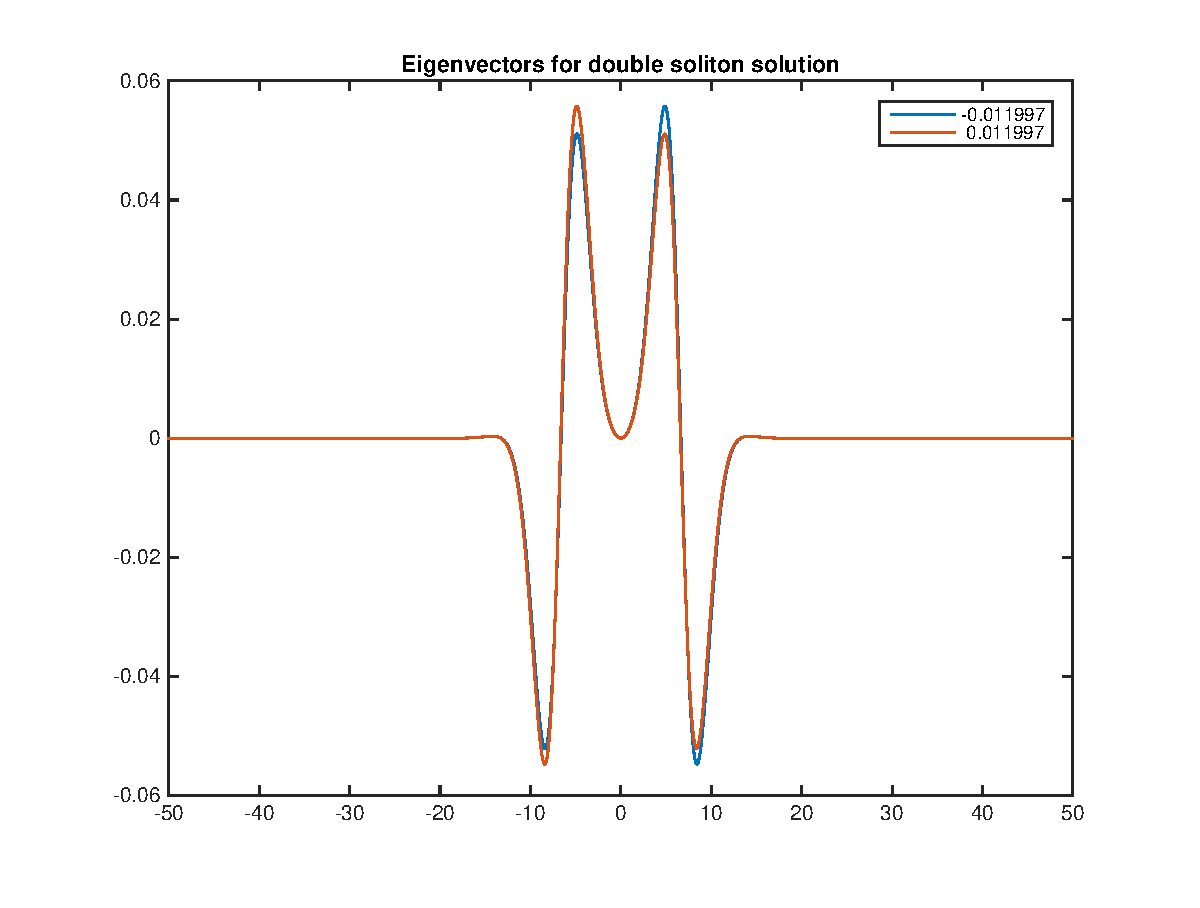
\includegraphics[width=8.5cm]{double1_FD50_vec.eps}
	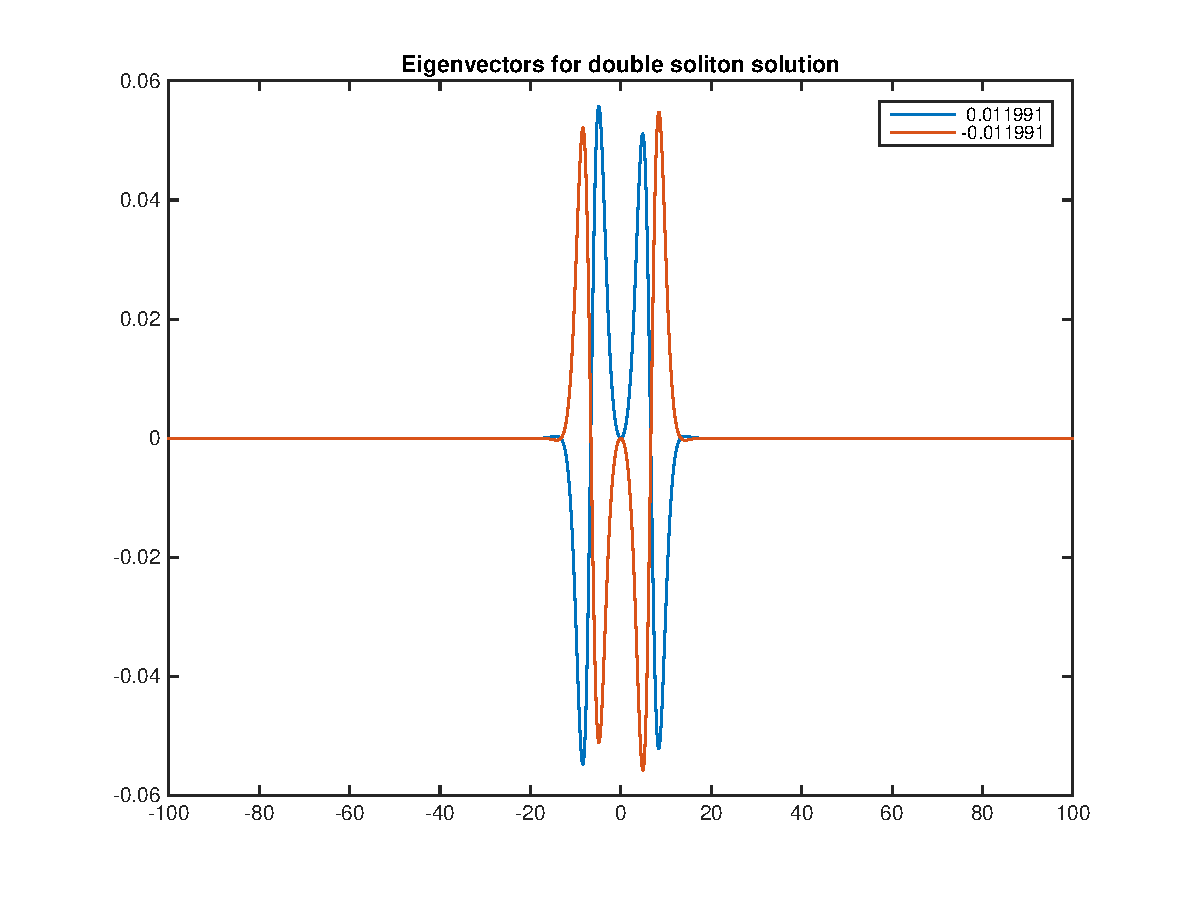
\includegraphics[width=8.5cm]{double1_FD100_vec.eps}
	\end{figure}

Eigenvalues are much closer this time: $\pm 0.011997$ for $L = 50$ and $0.011991$ for $L = 100$. For Fourier spectral method on domain scaled to $L = 50$, we get eigenvalues $\pm 0.01198$.

	\begin{figure}[H]
	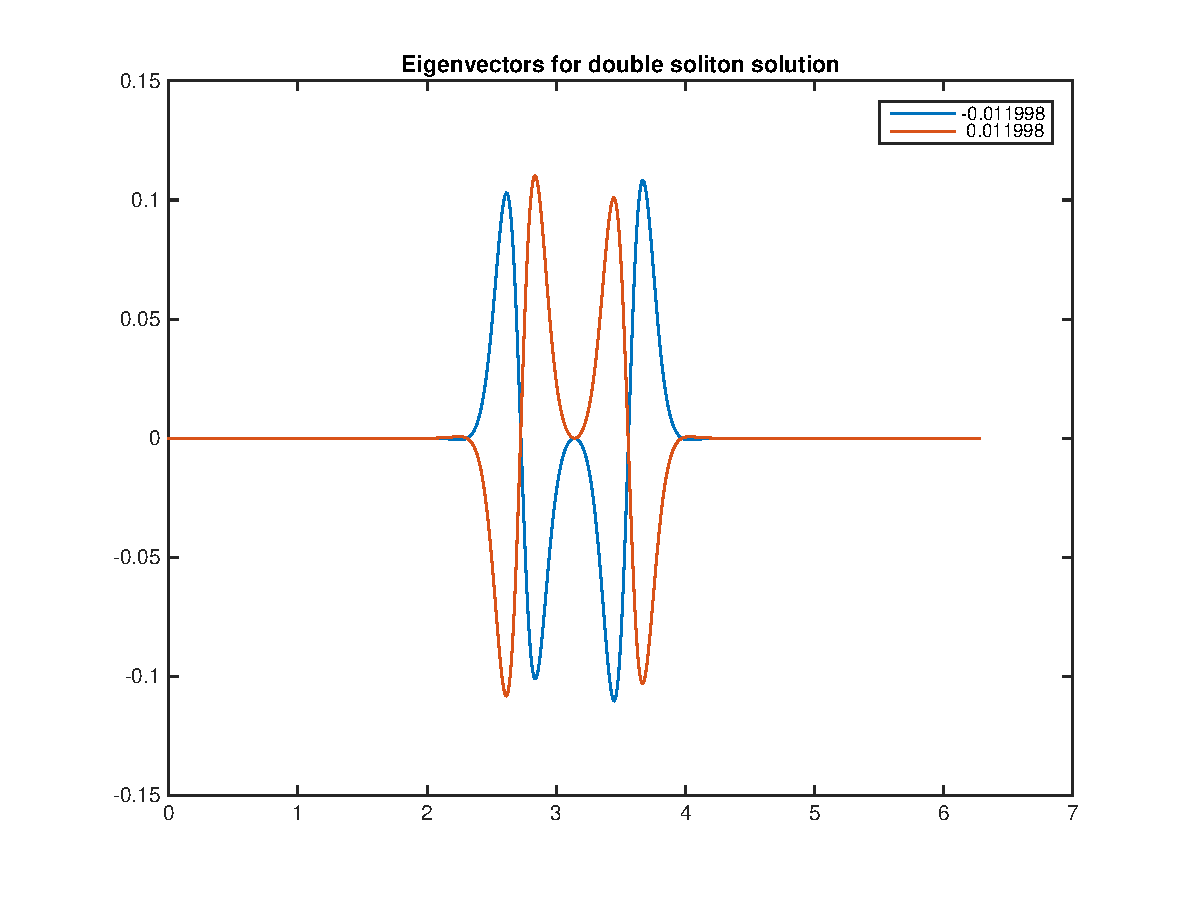
\includegraphics[width=8.5cm]{double1_Four50_vec.eps}
	\end{figure}

\section*{2 Feb 2017}
Numerical method for finite differences is now the following:
\begin{enumerate}
	\item Start with known solution, use half-wave with Neumann boundary conditions.
	\item Use continuation method to increase speed $c$ to above 1/4.
	\item Construct full wave from half-wave by reflection symmetry.
	\item Find max/mins of tail oscillations of full wave.
	\item Construct double pulse by joining at these max/mins.
	\item Take half-wave for double pulse, since fewer grid points and we have reflection symmetry. (Previously, we used full wave here).
	\item Run Newton solver on half-wave for double pulse.
	\item Use reflection symmetry to reconstruct full wave (after Newton solver run)/
	\item Use eigs/eig to numerically find eigenvalues/eigenvectors.
\end{enumerate}

Now we do this for double pulses joined at the first 3 min/maxes. (We could keep going, but could need to use a larger domain in that case, which requires more grid points). In all cases, the Newton solver converges. We find the min/maxes using calculus; the distance between subsequent min/maxes is the same as the expected frequency, so that checks out. 

\subsection*{Double pulse, joined at first min/max}
Plots of the half-wave for the double pulse.
	\begin{figure}[H]
	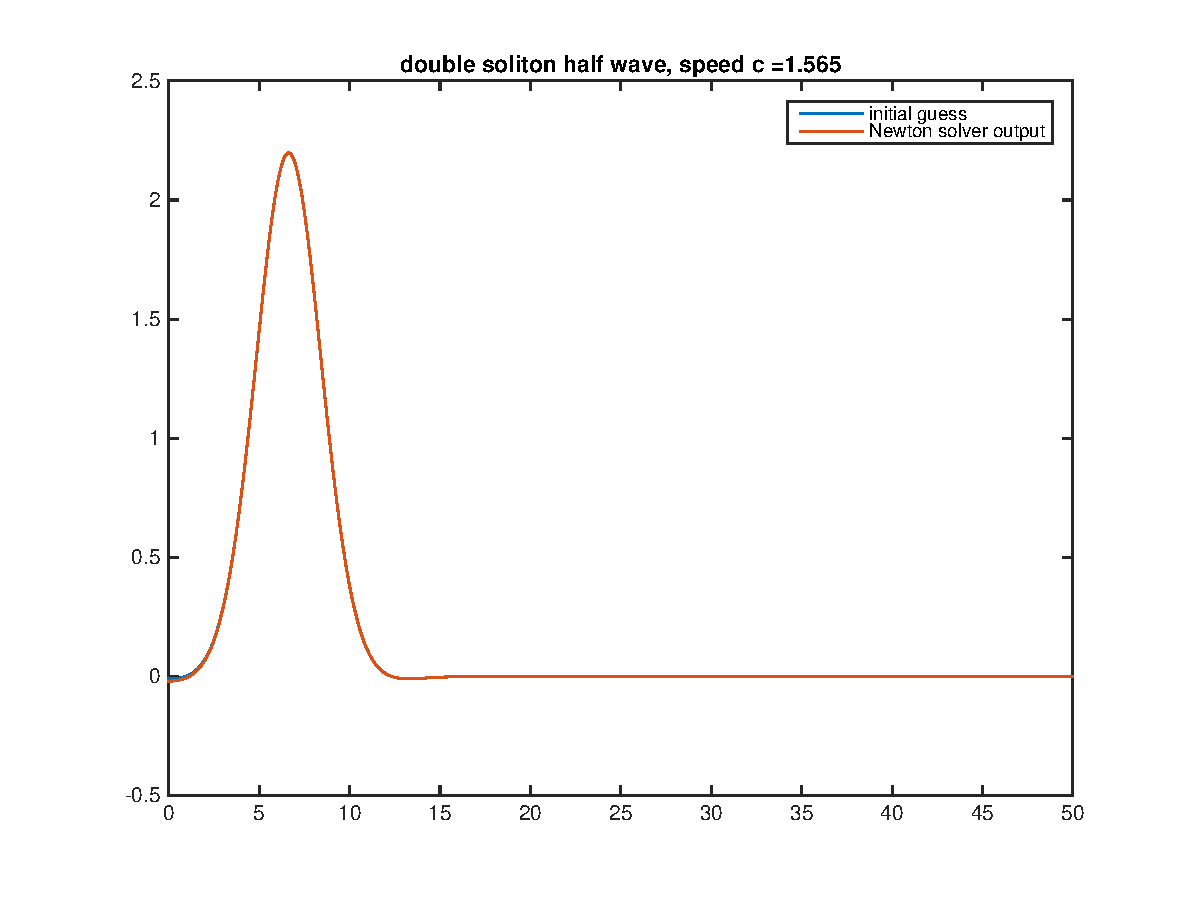
\includegraphics[width=8.5cm]{D1_fd50_half.eps}
	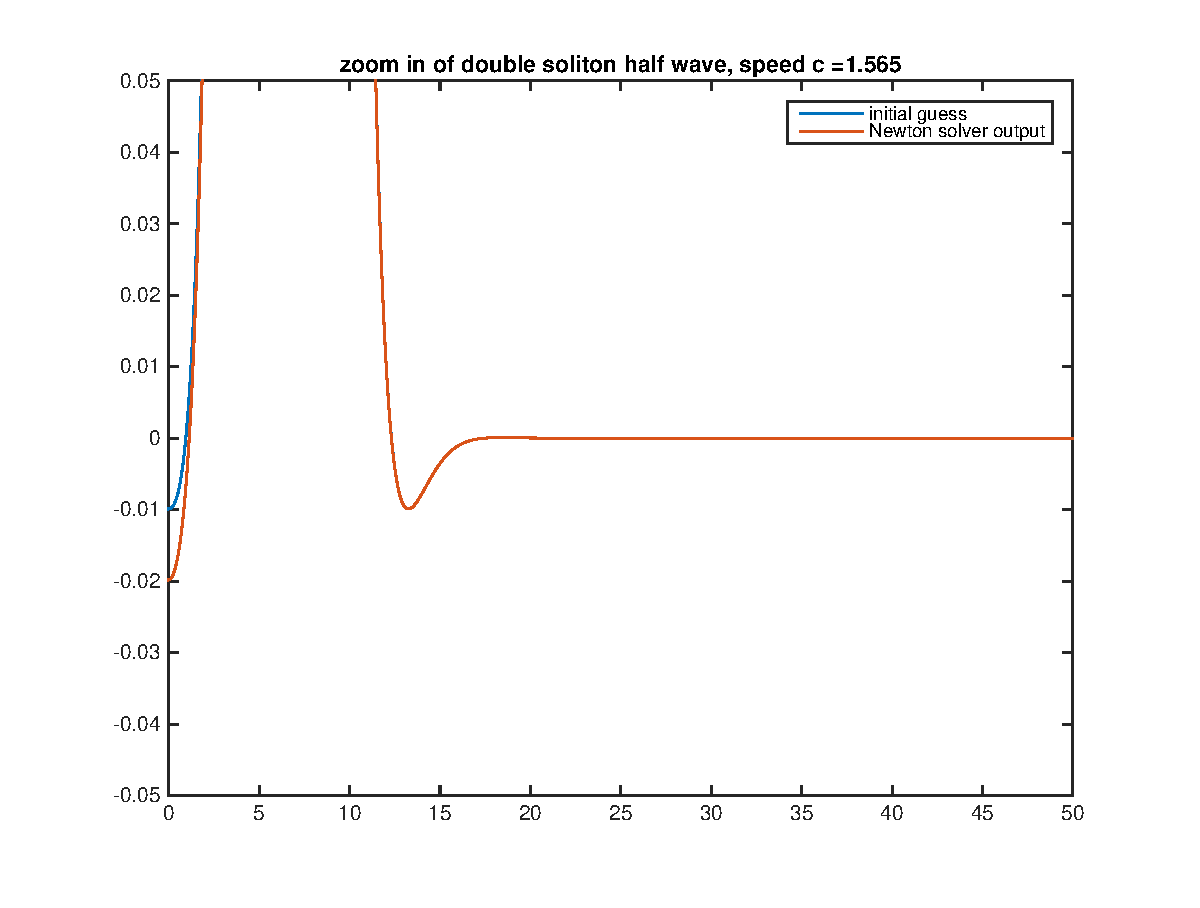
\includegraphics[width=8.5cm]{D1_fd50_half_zoom.eps}
	\end{figure}

Plot of eigenvalues for the double pulse.
	\begin{figure}[H]
	\includegraphics[width=8.5cm]{D1_fd50_val.eps}
	\end{figure}

We have four eigenvalues on the real axis (excluding the eigenvalue at 0): -0.00010209, 0.00010201, 0.011997, -0.011997. My guess is that the small ones should also be negatives of each other, but that they are not due to limitations in the numerical methods.

\subsection*{Double pulse, joined at second min/max}
Plots of the half-wave for the double pulse.
	\begin{figure}[H]
	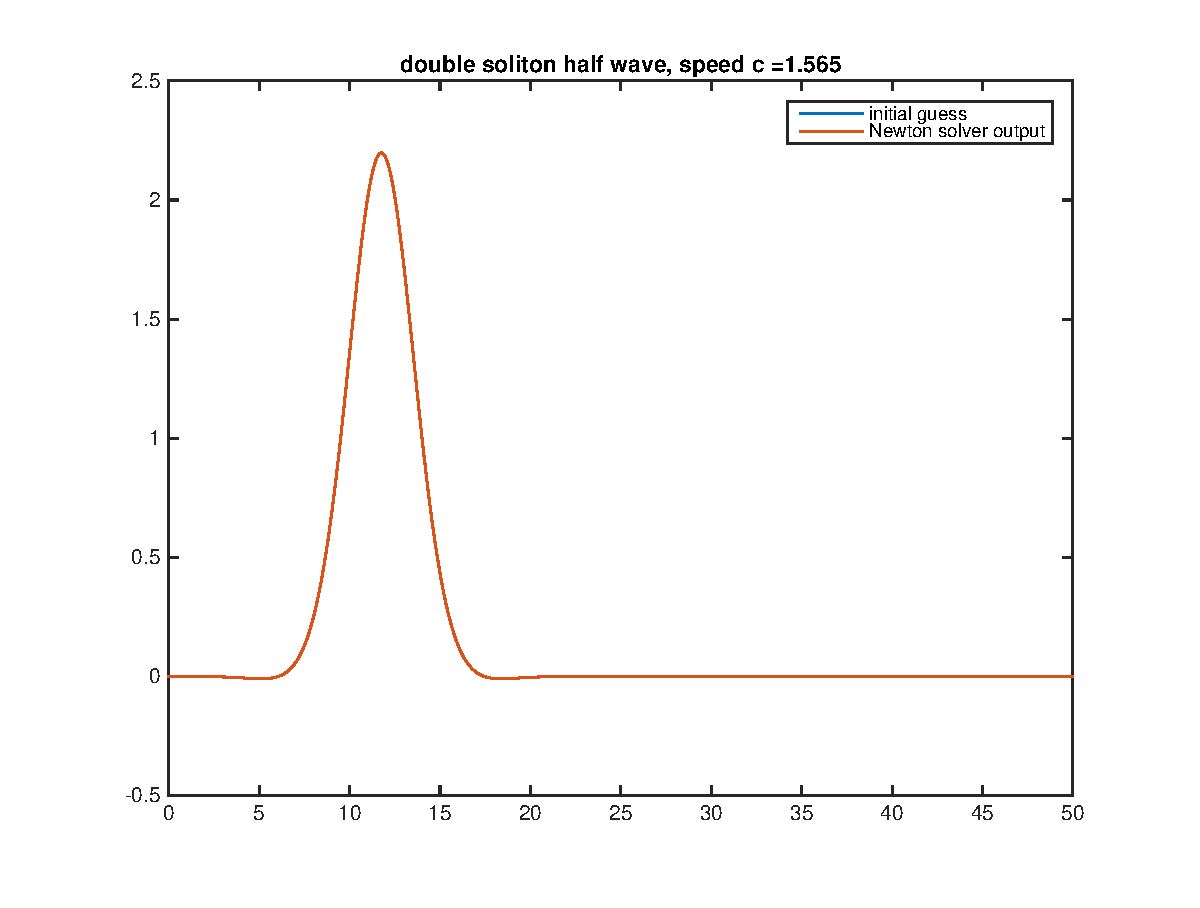
\includegraphics[width=8.5cm]{D2_fd50_half.eps}
	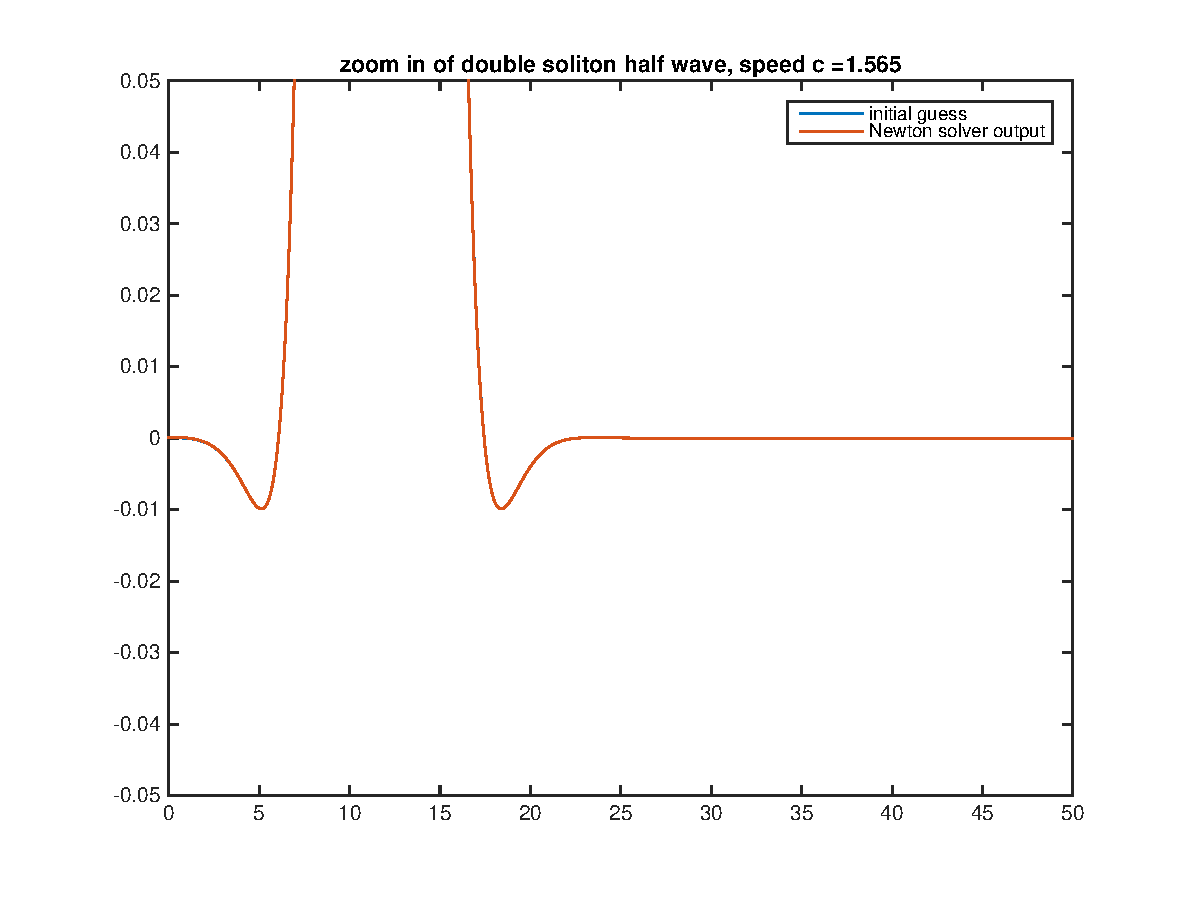
\includegraphics[width=8.5cm]{D2_fd50_half_zoom.eps}
	\end{figure}

Plot of eigenvalues for the double pulse.
	\begin{figure}[H]
	\includegraphics[width=8.5cm]{D2_fd50_val.eps}
	\end{figure}

We have four eigenvalues on the real axis (excluding the eigenvalue at 0): 2.8826e-04, -2.8816e-04, 1.9105e-05, -1.9189e-05. 

\subsection*{Double pulse, joined at third min/max}
Plots of the half-wave for the double pulse.
	\begin{figure}[H]
	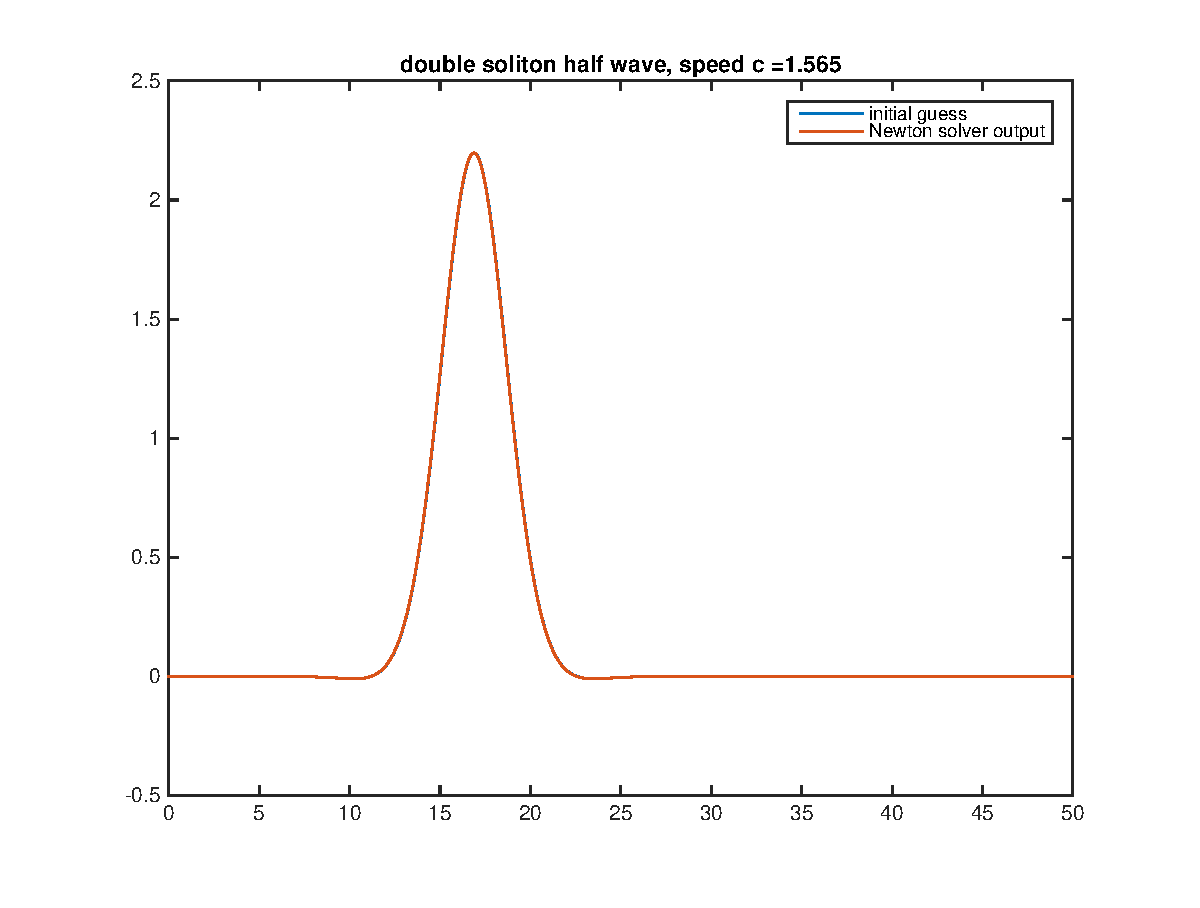
\includegraphics[width=8.5cm]{D3_fd50_half.eps}
	\includegraphics[width=8.5cm]{D3_fd50_half_zoom.eps}
	\end{figure}

Plot of eigenvalues for the double pulse.
	\begin{figure}[H]
	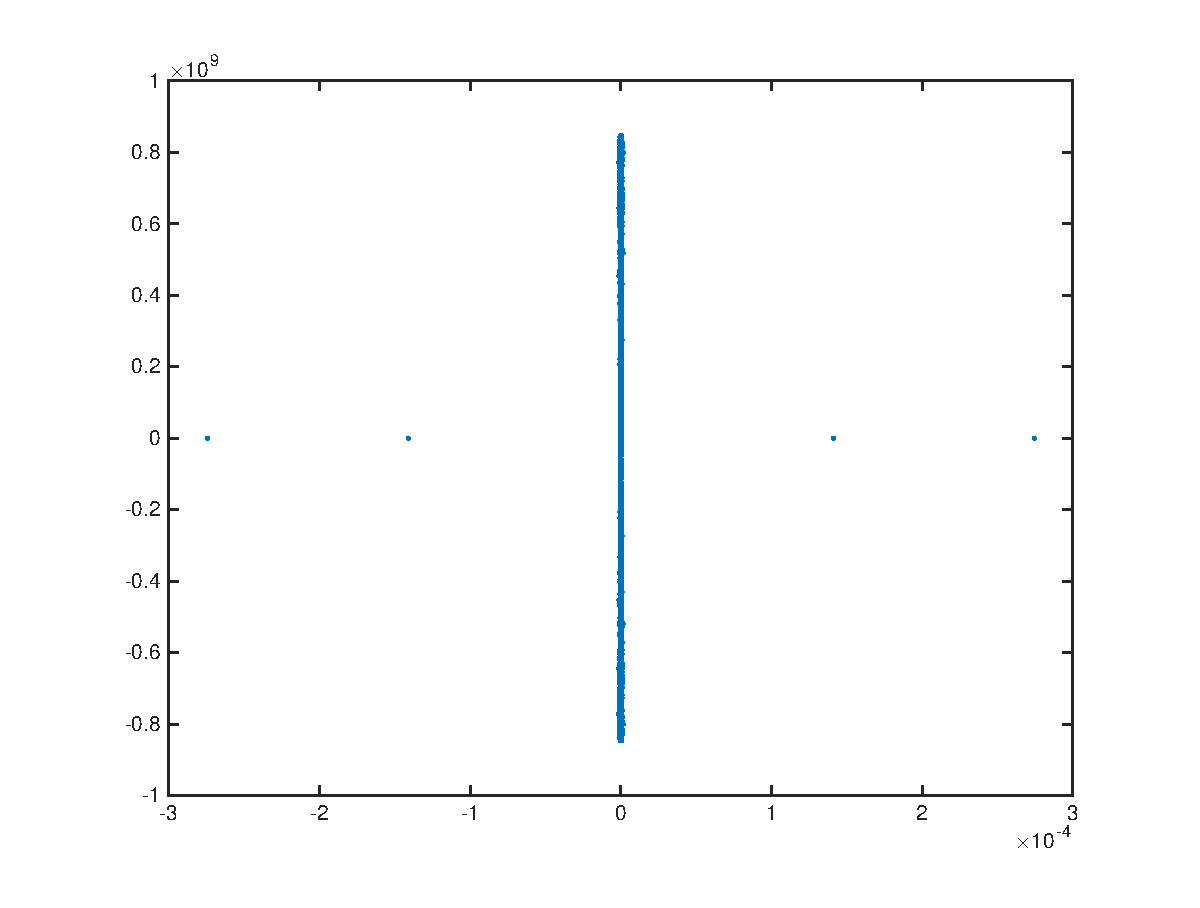
\includegraphics[width=8.5cm]{D3_fd50_val.eps}
	\end{figure}

We have four eigenvalues on the real axis (excluding the eigenvalue at 0): 2.7429e-04, -2.7431e-04, 1.4112e-04, -1.4109e-04.

\section*{6 Feb 2017}
Repeat the above with $L = 100$ and 2000 grid points for the half-wave (3999 for the full wave). Eigenvalue problem for linearization can be successfully solved numerically (i.e. without breaking down due to too short a domain) for double pulses joined at at least the first 10 (!) min/max. Graphs of just the eigenvalues are below. Plots are all labeled 1st min/max, but they are in order from 1st to 10th.

	\begin{figure}[H]
	\includegraphics[width=8.5cm]{L100eigs1.eps}
	\includegraphics[width=8.5cm]{L100eigs2.eps}
	\end{figure}
	\begin{figure}[H]
	\includegraphics[width=8.5cm]{L100eigs3.eps}
	\includegraphics[width=8.5cm]{L100eigs4.eps}
	\end{figure}
	\begin{figure}[H]
	\includegraphics[width=8.5cm]{L100eigs5.eps}
	\includegraphics[width=8.5cm]{L100eigs6.eps}
	\end{figure}
	\begin{figure}[H]
	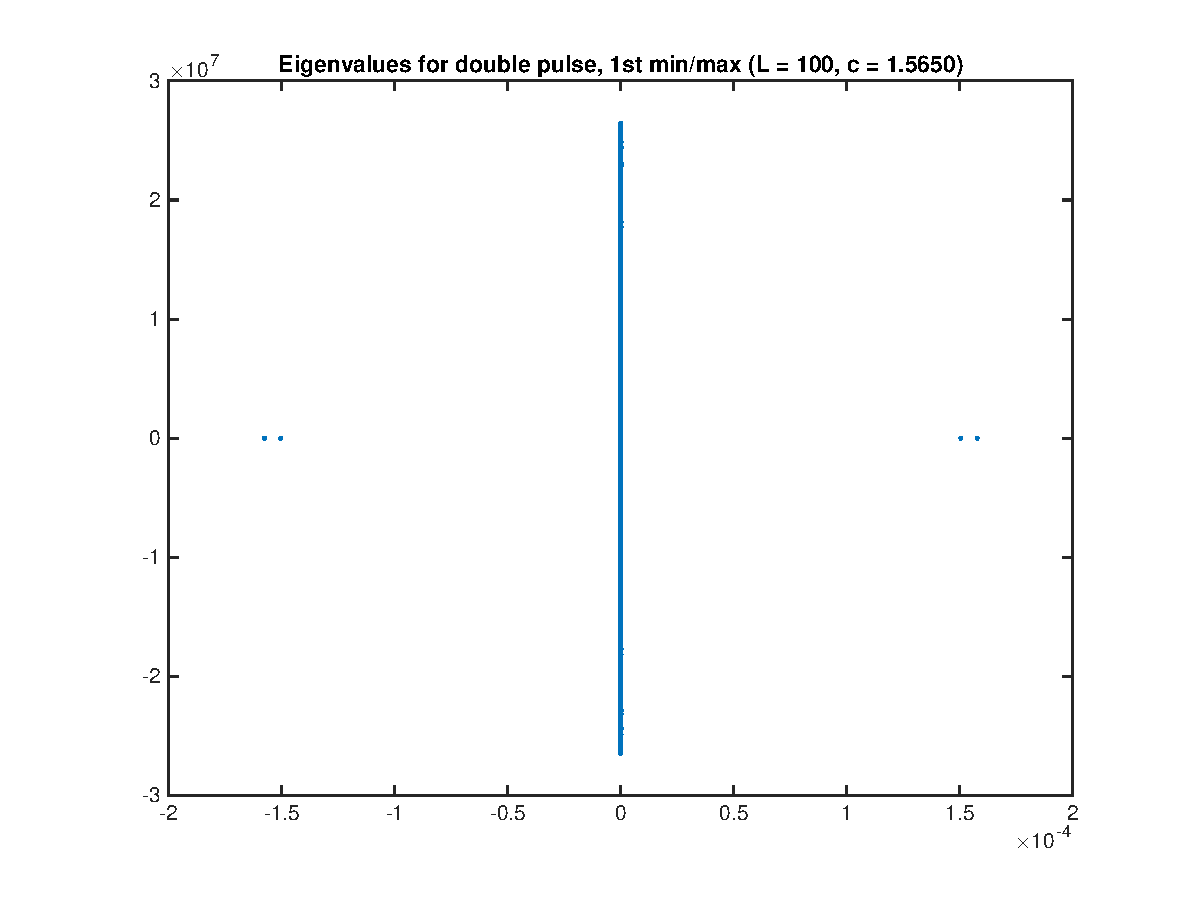
\includegraphics[width=8.5cm]{L100eigs7.eps}
	\includegraphics[width=8.5cm]{L100eigs8.eps}
	\end{figure}
	\begin{figure}[H]
	\includegraphics[width=8.5cm]{L100eigs9.eps}
	\includegraphics[width=8.5cm]{L100eigs10.eps}
	\end{figure}



\end{document}

